\begin{frame}\frametitle{\footnotesize{$P_T^{\gamma}$ Distribution of $W\gamma\rightarrow\mu\nu\gamma$ Candidates (ECal Barrel Only)}}

\begin{minipage}[b]{0.49\textwidth}
   \begin{figure}[htb]
    \begin{center}
       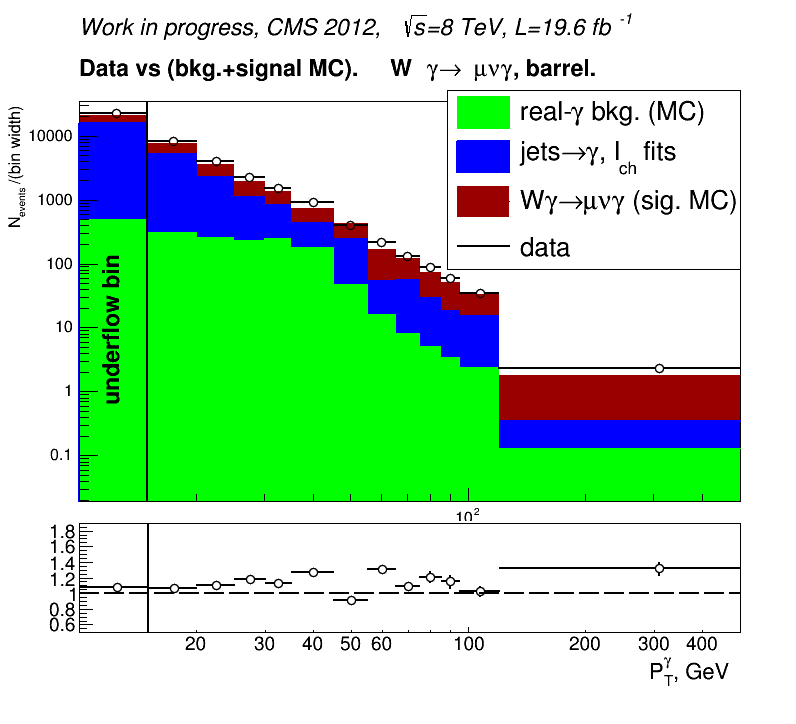
\includegraphics[width=0.85\textwidth]{../figs/ForPresentation/forDefense_DATAvsBKGplusSIG_CHISO_Wg_Muon.png}\\
       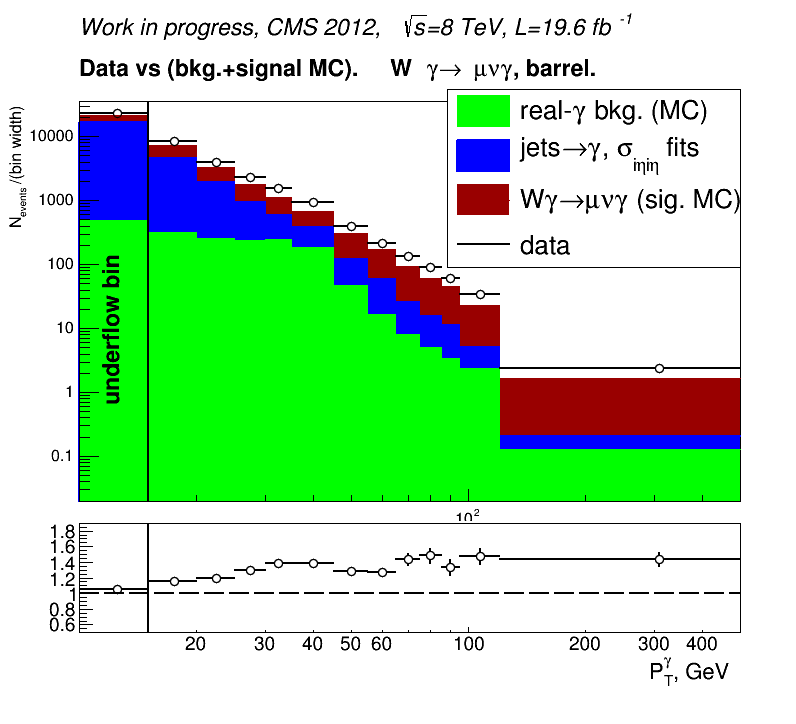
\includegraphics[width=0.85\textwidth]{../figs/ForPresentation/forDefense_DATAvsBKGplusSIG_SIHIH_Wg_Muon.png}\\
    \end{center}
  \end{figure}
\end{minipage}%
\begin{minipage}[b]{0.49\textwidth}
\tiny
{\bfseries{Left:}} $P_T^{\gamma}$ distribution {\bfseries{before}} the background subtraction. Jets$\rightarrow\gamma$ background is estimated using fits of $I_{ch}^{\gamma}$ (top) and $\sigma_{i\etai\eta}^{\gamma}$ (bottom) templates.\\
-\\
{\bfseries{Right:}} $P_T^{\gamma}$ distribution {\bfseries{after}} the background subtraction. Signal $P_T^{\gamma}$ distributions obtained using fits of $I_{ch}^{\gamma}$ vs $\sigma_{i\etai\eta}^{\gamma}$ templates vs signal MC simulation.\\
  \begin{figure}[htb]
    \begin{center}
       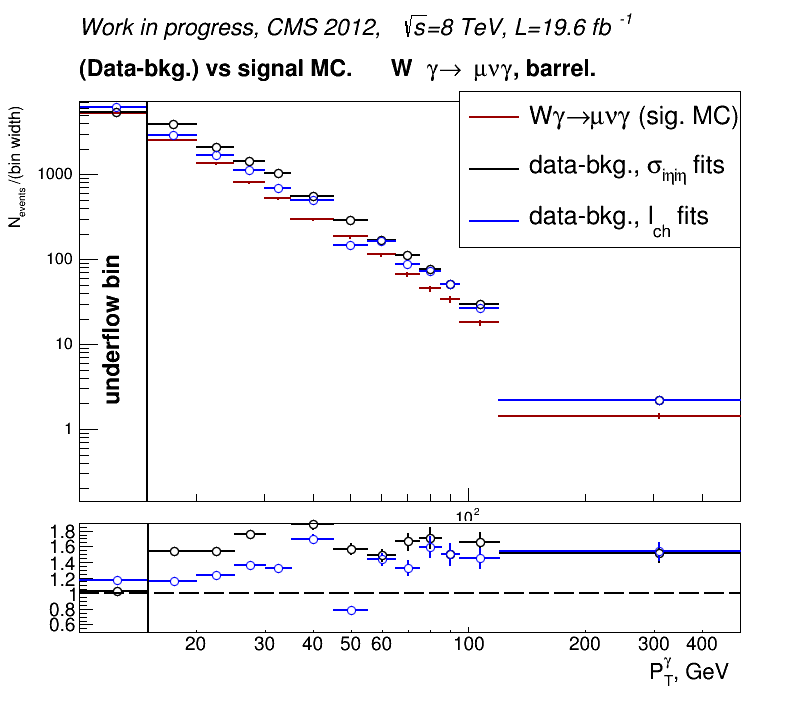
\includegraphics[width=0.98\textwidth]{../figs/ForPresentation/forDefense_DATAminusBKG_Wg_Muon.png}\\
    \end{center}
  \end{figure}
\end{minipage}
\end{frame}%{$jets \rightarrow \gamma$ Background Subtraction. Plots, W$\gamma$}


